\documentclass{beamer}
\usetheme{Berlin}
\usecolortheme{beaver}
\usepackage{graphicx}
\usepackage[export]{adjustbox}
\usepackage{tikz}
\usetikzlibrary{arrows}
\usepackage{amsmath}
\usepackage{lmodern}% http://ctan.org/pkg/lm
\usepackage{mathtools}
\usefonttheme{professionalfonts}

\title{Chapters 9.3-9}
\subtitle{}
\author[Riccardo \and Eren]{Riccardo~Miccini\inst{1} \and Eren~Can~\inst{1}}
\institute[DTU]
{
	\inst{1}
	Technical University of Denmark\\
	Digital Communication
}
\date{\today}
\subject{Digital Communication}

\tikzstyle{int}=[draw, fill=blue!20]
\tikzstyle{every node}=[font=\tiny]

\begin{document}
\frame{\titlepage}

% ch 9.3
\begin{frame}
	\frametitle{Modulation Schemes not Requiring Coherent References}
	\begin{itemize}
		\item .
	\end{itemize}
\end{frame}

\begin{frame}
	\frametitle{Differential Phase-Shift Keying  (DPSK)}
	\begin{itemize}
		\item .
	\end{itemize}
\end{frame}


% ch 9.5
\begin{frame}
	\frametitle{Comparison of Digital Modulation Systems}
	\begin{itemize}
		\item .
	\end{itemize}
\end{frame}


% ch 9.7
\begin{frame}
	\frametitle{Multipath Interference (1)}
	\begin{itemize}
		\item Additive Gaussian noise is not sufficient to accurately model the transmission channel
		\item Other sources of degradation:
		\begin{itemize}
			\item bandwidth limiting by the channel
			\item impulse noise (lightnings, switching)
			\item RF interference from other transmitters
			\item \emph{multipath interference} from signal reflections and scattering
		\end{itemize}
	\end{itemize}
\end{frame}

\begin{frame}
	\frametitle{Multipath Interference (2)}
	\begin{itemize}
		\item Two-way multipath model: $ y(t) = s_d(t) + \beta s_d(t - \tau_m) + n(t) $
		\begin{description}
			\item[$ n(t) $] Gaussian noise component
			\item[$ s_d(t) $] Signal from the direct path
			\item[$ \beta $] Gain of secondary path component
			\item[$ \tau_m $] Time delay of secondary path component
		\end{description}
		\item For binary phase-shift keying signals: $ s_d(t) - Ad(t)\cos(\omega_c t) $
		\begin{description}
			\item[$ d(t) $] Data stream (sequence of $ \pm1 $ rectangular pulses) of width T
			\item[$ \omega_c $] Carrier frequency
		\end{description}
	\end{itemize}
\end{frame}

\begin{frame}
	\frametitle{Multipath Interference (3)}
	\begin{itemize}
		\item Input of the integrator at the receiving end: $ x(t) = LP\{2y(t)\cos(\omega_c t)\} = Ad(t) + \beta Ad(t - \tau_m)\cos(\omega_c \tau_m) + n_c(t) $
		\item Two scenarios:
		\begin{description}
			\item[$ \tau_m/T \cong 0 $] The original and reflected signals are almost congruent, so $ \omega_c \tau_m $ is uniformly distributed in $ [-\pi, \pi] $. When many reflection components are considered, the envelope of the signal assumes a Rayleigh or Ricean distribution
			\item[$ 0 < \tau_m/T \leq 1 $] Adjacent bits in the original and reflected signals overlap; inter-symbol interference appears
		\end{description}
	\end{itemize}
\end{frame}

\begin{frame}
	\frametitle{Multipath Interference - second scenario (1)}
	\begin{itemize}
		\item Four equally likely cases; total probability of error is: $ P_E = \frac{1}{4}[P(E|++) + P(E|-+) + P(E|+-) + P(E|--)] $
		\item Noise on the integrator integrator out is Gaussian-distributed with $ \mu = 0 $ and $ \omega^2_n = N_0T $
		\item Due to the symmetric nature of the overlapping bits and Gaussian probability density function, only two cases need to be computed
		\begin{itemize}
			\item $ P(E|++) = P(E|--) = Q\left[\sqrt{\frac{2E_b}{N_0}}(1+\delta)\right] $
			\item $ P(E|+-) = P(E|-+) = Q\left[\sqrt{\frac{2E_b}{N_0}}\left((1+\delta) - \frac{2\delta\tau_m}{T}\right)\right] $
		\end{itemize}
		\item After substituting the cases above into the matching ones: $ P_E = \frac{1}{2}Q\left[\sqrt{2z_0}(1+\delta)\right] + \frac{1}{2}Q\left[\sqrt{2z_0}\left((1+\delta) - \frac{2\delta\tau_m}{T}\right)\right] $
	\end{itemize}
\end{frame}

\begin{frame}
	\frametitle{Multipath Interference - second scenario (2)}
	\begin{itemize}
		\item Overal probability of error changes with $ z_0 = \frac{E_b}{N_0} = \frac{A^2T}{2N_0} $
	\end{itemize}
	\begin{figure}
		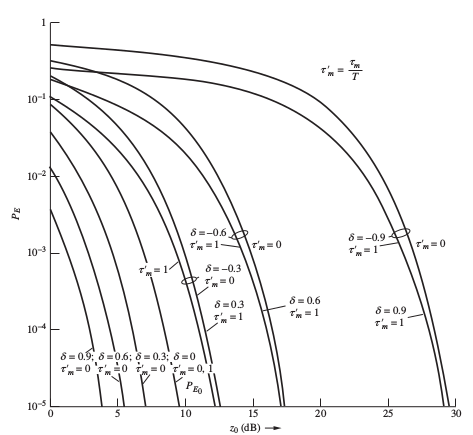
\includegraphics[width=\textwidth, height=0.7\textheight, keepaspectratio]{pe_vs_z0.png}
	\end{figure}
\end{frame}


% ch 9.9
\begin{frame}
	\frametitle{Equalization}
	\begin{itemize}
		\item Equalization is used in telecommunication to reverse the signal degradation caused by multipath propagation and bandwidth limitations
		\item Simplest form of equalization consists in an inverse filter - \emph{Tapped-delay-line filter}
		\item Two ways of determining the filter coefficients:
		\begin{itemize}
			\item zero-forcing
			\item mean-square error
		\end{itemize}
	\end{itemize}
\end{frame}

\begin{frame}
	\frametitle{Equalization by Zero Forcing}
	\begin{itemize}
		\item Impulse response of equalized output: $ p_{eq}(mT) = \sum_{n=-N}^N {\alpha_n p_c((m-n)T)} \Rightarrow [P_{eq}]=[P_c][A] $
		\item $ [P_{eq}] $ is a column vector composed of: N zeros, 1, N zeros
		\item Equalizarion filter coefficient matrix: $ [A]_{opt} = [P_c]^{-1}[P_{eq}] $
		\item Multiplying by $ [P_{eq}] $ corresponds to picking the middle column of matrix $ [P_c]^{-1} $
	\end{itemize}
\end{frame}

\begin{frame}
	\frametitle{Equalization by Minimum Mean-Squared Error (1)}
	\begin{itemize}
		\item Obtain filter coefficients that minimize the difference between the output of the equalizer and the actual output: $ \varepsilon = E\left\{[z(t) - d(t)]^2\right\} = minimum $
		\begin{itemize}
			\item $ z(t) $ is the equalizer output response (incl. noise): $ z(t) = \sum_{n=-N}^N {\alpha_n p_c((m-n)T)} $
			\item $ d(t) $ is the desired response
		\end{itemize}
	\end{itemize}
\end{frame}

\begin{frame}
	\frametitle{Equalization by Minimum Mean-Squared Error (2)}
	\begin{itemize}
		\item $ \varepsilon $ is concave and can be minimized by derivation: $ \frac{\delta\varepsilon}{\delta\alpha_m} = 0 = 2E\left\{[z(t) - d(t)] \frac{\delta z(t)}{\delta\alpha_m} \right\} $
		\item Substituting $ z(t) $ gives the following conditions (in terms of cross-correlation): $ R_{yz}(m\Delta) = R_{yd}(m\Delta) = 0 $
		\begin{itemize}
			\item $ R_{yz}(\tau) = E[y(t)z(t + \tau)] $
			\item $ R_{yd}(\tau) = E[y(t)d(t + \tau)] $
		\end{itemize}
		\item In terms of matrices: $ [R_{yy}][A]_{opt} = [R_{yd}] $
		\item Solving for the filter taps: $ [A]_{opt} = [R_{yy}]^{-1}[R_{yd}] $
	\end{itemize}
\end{frame}

\begin{frame}
	\frametitle{Tap Weight Ajustment (LMS Algorithm) (1)}
	\begin{itemize}
		\item How to obtain $ d(t) $
		\begin{enumerate}
			\item Periodically send known data sequence used for weight adjustment
			\item Use method 1 for first guess and then use detected data (\emph{decision-directed} mode)
		\end{enumerate}
		\item Apply gradient descent to initial weight values ($ [A]^{(0)} $): $ [A]^{(k+1)} = [A]^{(k)} + \frac{1}{2}\mu [-\nabla\varepsilon^{(k)}] $
		\begin{description}
			\item[$ k $] iteration of weights calculation
			\item[$ \nabla\varepsilon $] slope of error surface
			\item[$ \mu $] size of the step
		\end{description}
	\end{itemize}
\end{frame}

\begin{frame}
	\frametitle{Tap Weight Ajustment (LMS Algorithm) (2)}
	\begin{itemize}
		\item Alternative approach (Least-Mean-Square): $ \alpha^{(k+1)}_m = \alpha^{(k)}_m - \mu y[(k - m)\Delta] \epsilon(k\Delta) $
		\item $ \epsilon(k\Delta) $ is the error given by $ y_{eq}(k\Delta) - d(k\Delta) $
		\begin{description}
			\item[$ y_{eq}(k\Delta) $] equalization filter output
			\item[$ d(k\Delta) $] data sequence used for training
		\end{description}
	\end{itemize}
\end{frame}

\end{document}
